


\chapter{Introduction}

The Python script \texttt{dash-lineplot.py} is a general plotting utility that aids in visualisation of captured or recorded data. It reads an Excel configuration file and forms a set of Dash data structures in \ac{HTML} pages. A Dash portal is created where the \ac{HTML} pages are served via a Flask server.
The user has full control of the graph sets that are rendered on the pages.
Figure~\ref{fig:examplePage} shows an example of the Dash portal with different graph sets being rendered on several tabs.


\begin{figure}[h]
\centering
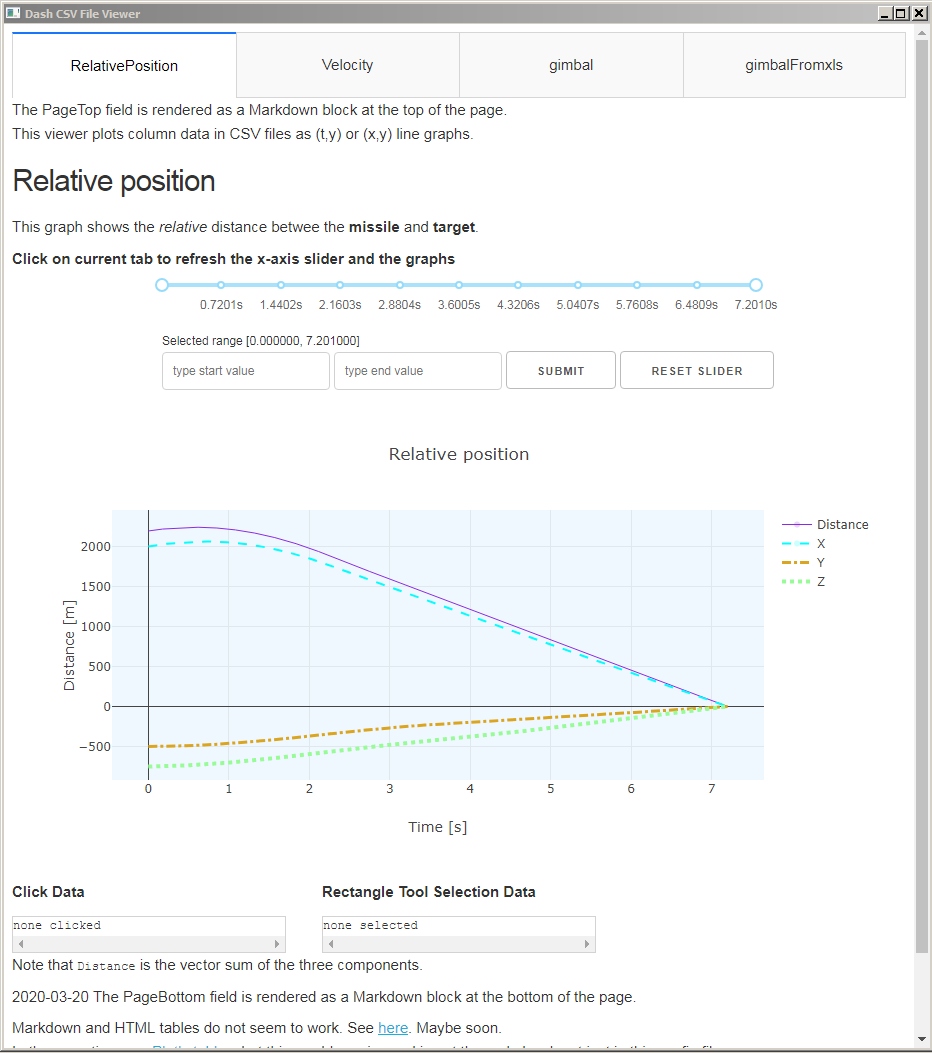
\includegraphics[width=0.70\textwidth]{pic/examplePage}
\caption{Example pages rendered by the dash-lineplot.py utility Python script.
\label{fig:examplePage}}
\end{figure}
